\appendix
%\addcontentsline{toc}{section}{Appendices}
\section{Appendices}
 \pagenumbering{roman}
 \subsection{Stewart Platform and Wind Tunnel Configurations}
 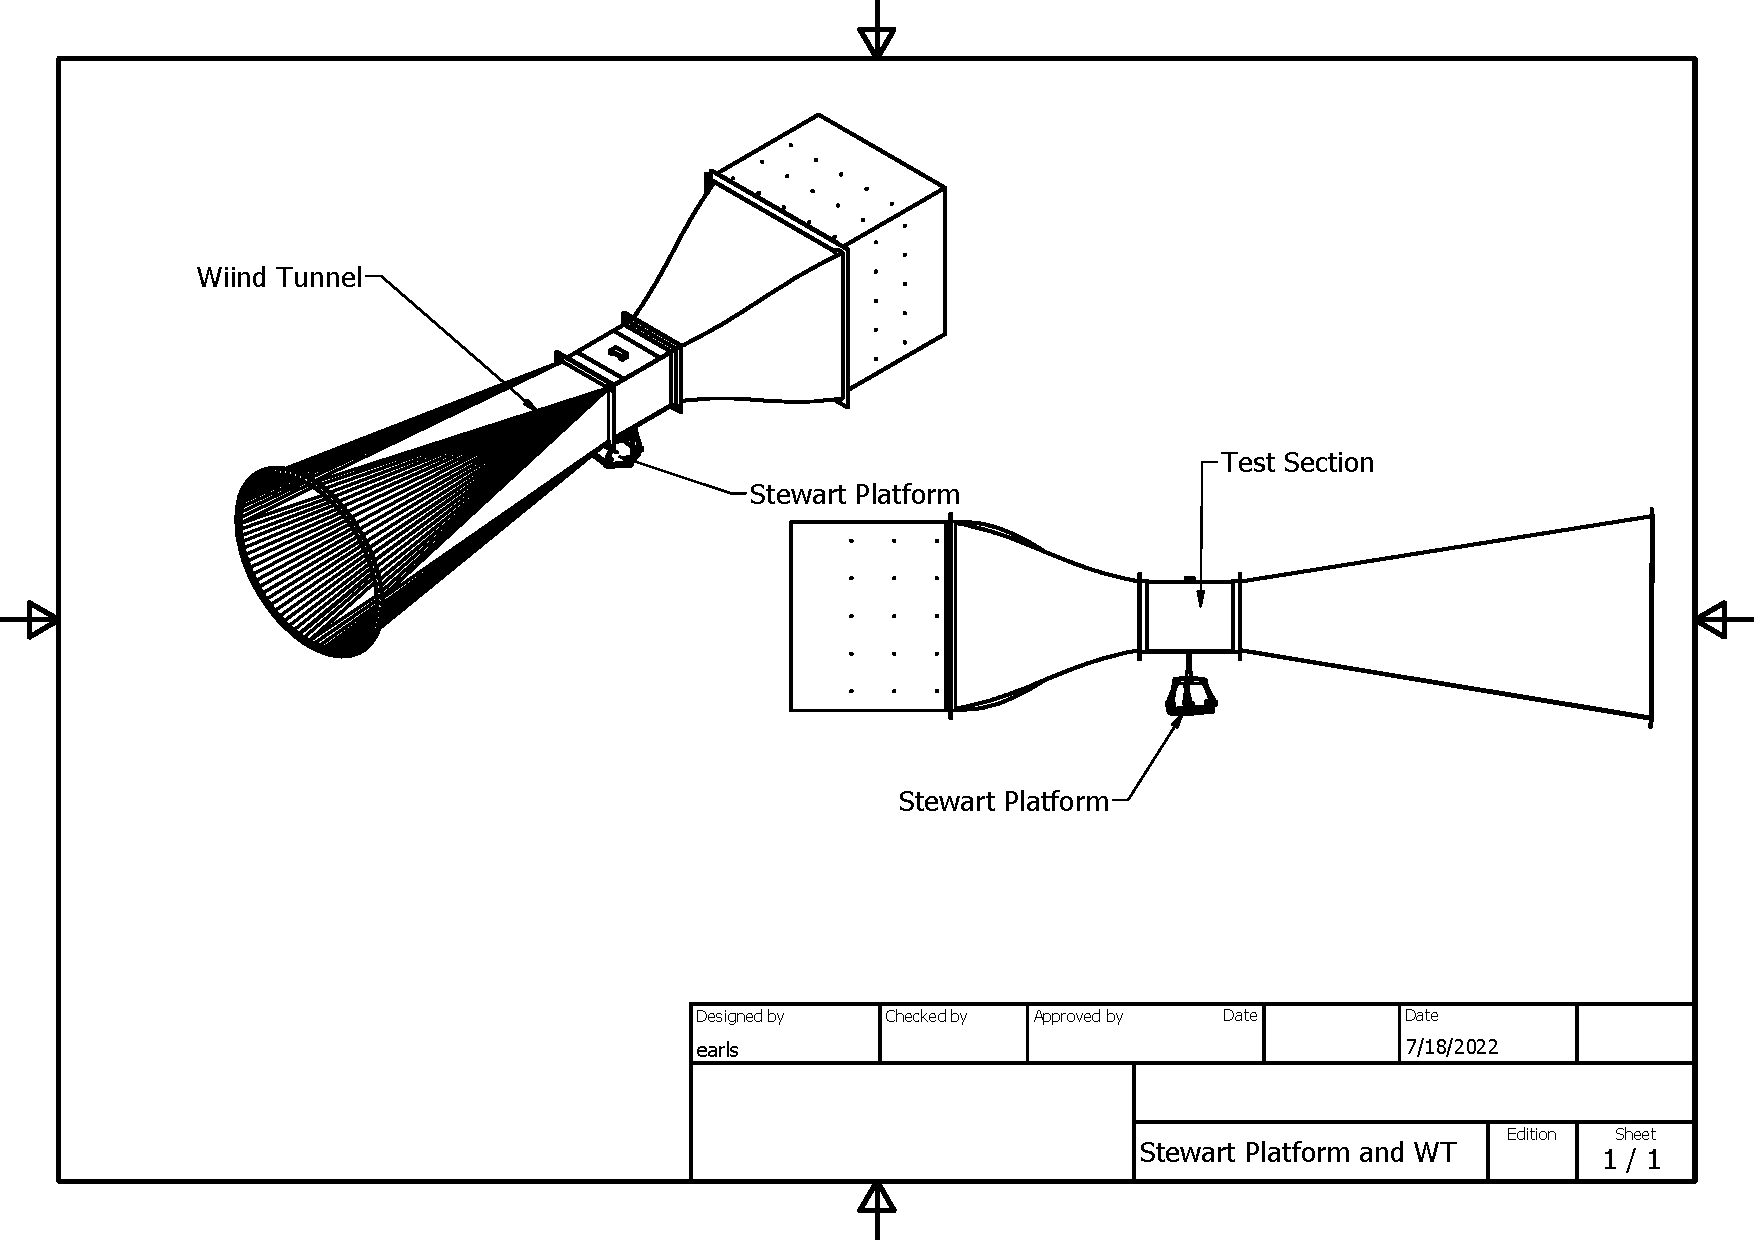
\includepdf[pages=-]{Wind Tunnel Assembly + Stewart}
 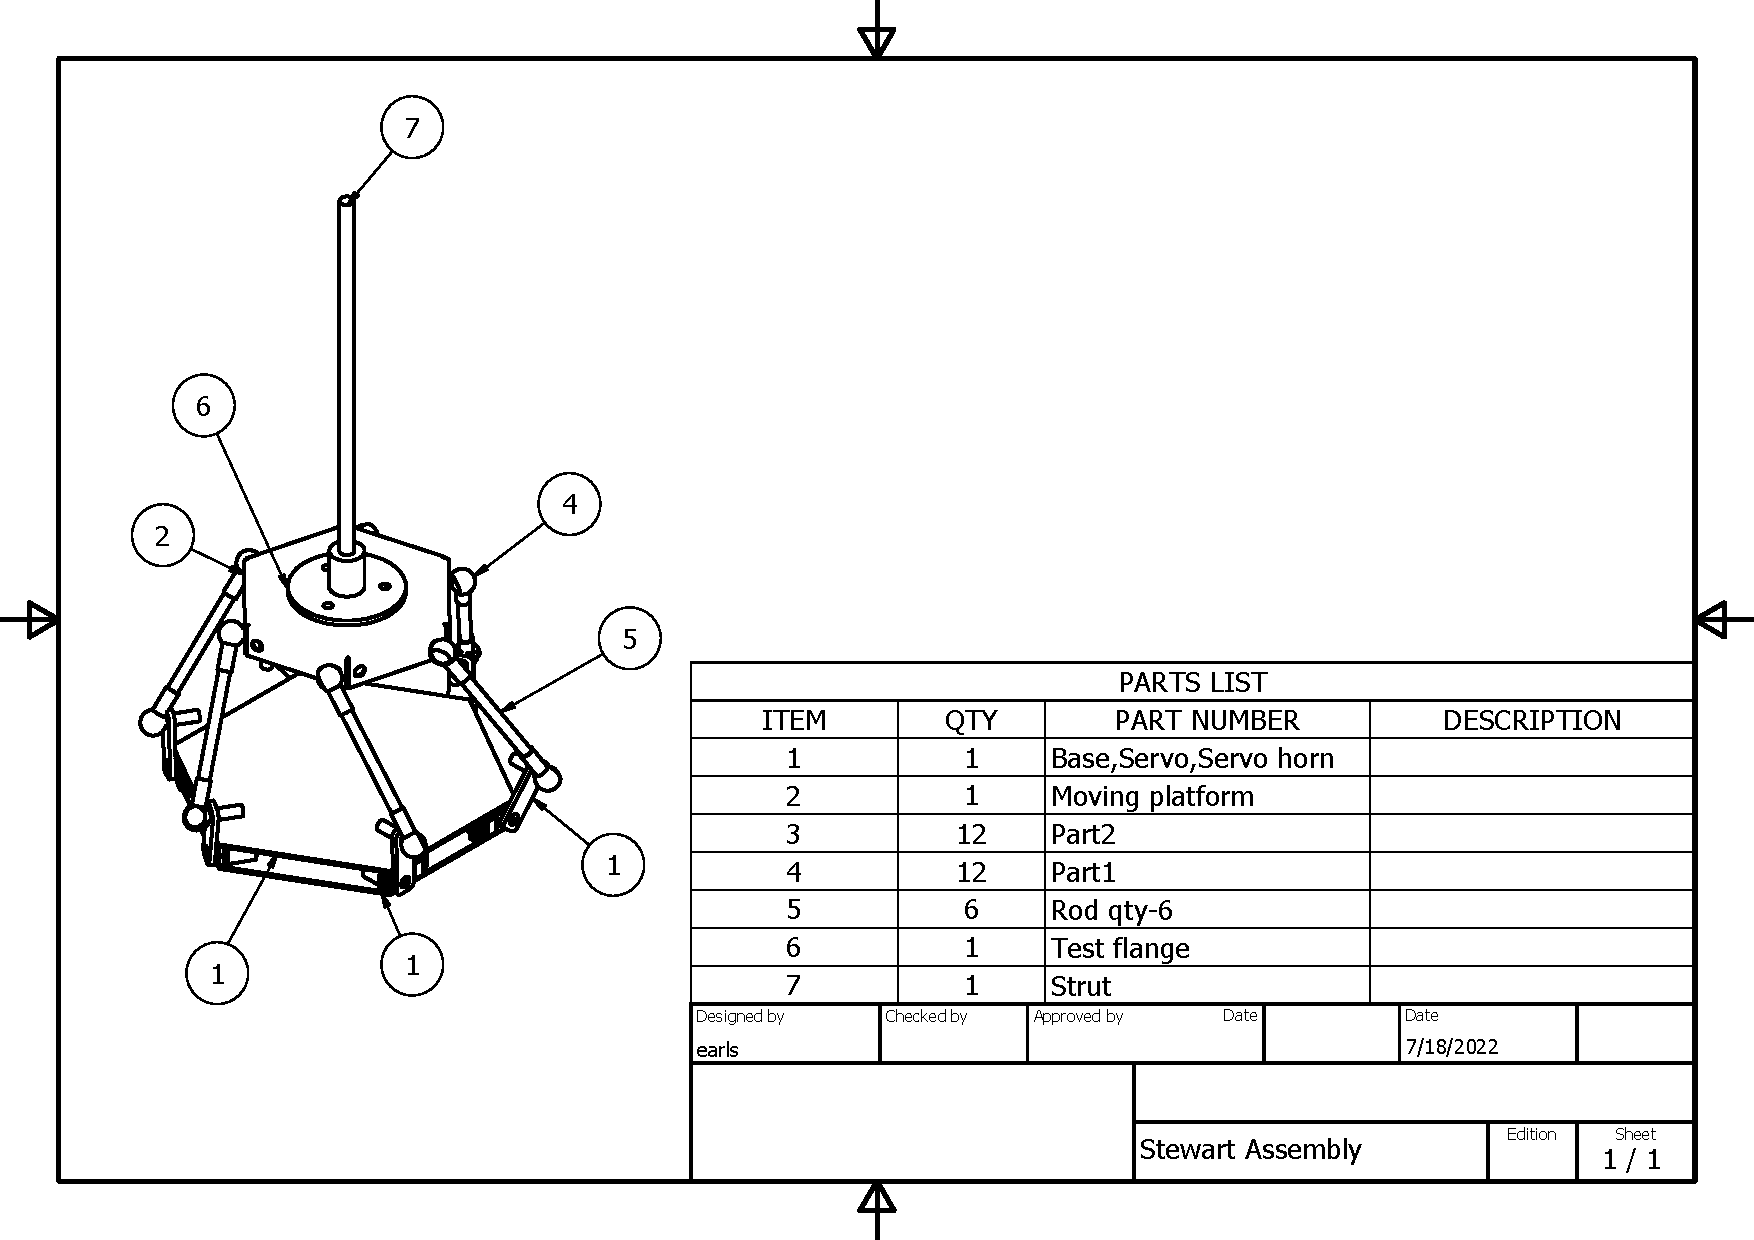
\includepdf[pages=-]{Assemby 3 2}
 \subsection{Budget and Timeplan}
 \subsubsection{Provisional Budget}
 \begin{center}
 \begin{table}[!h]
 \centering
 \caption{Proposed budget}
 \paragraph{ }
 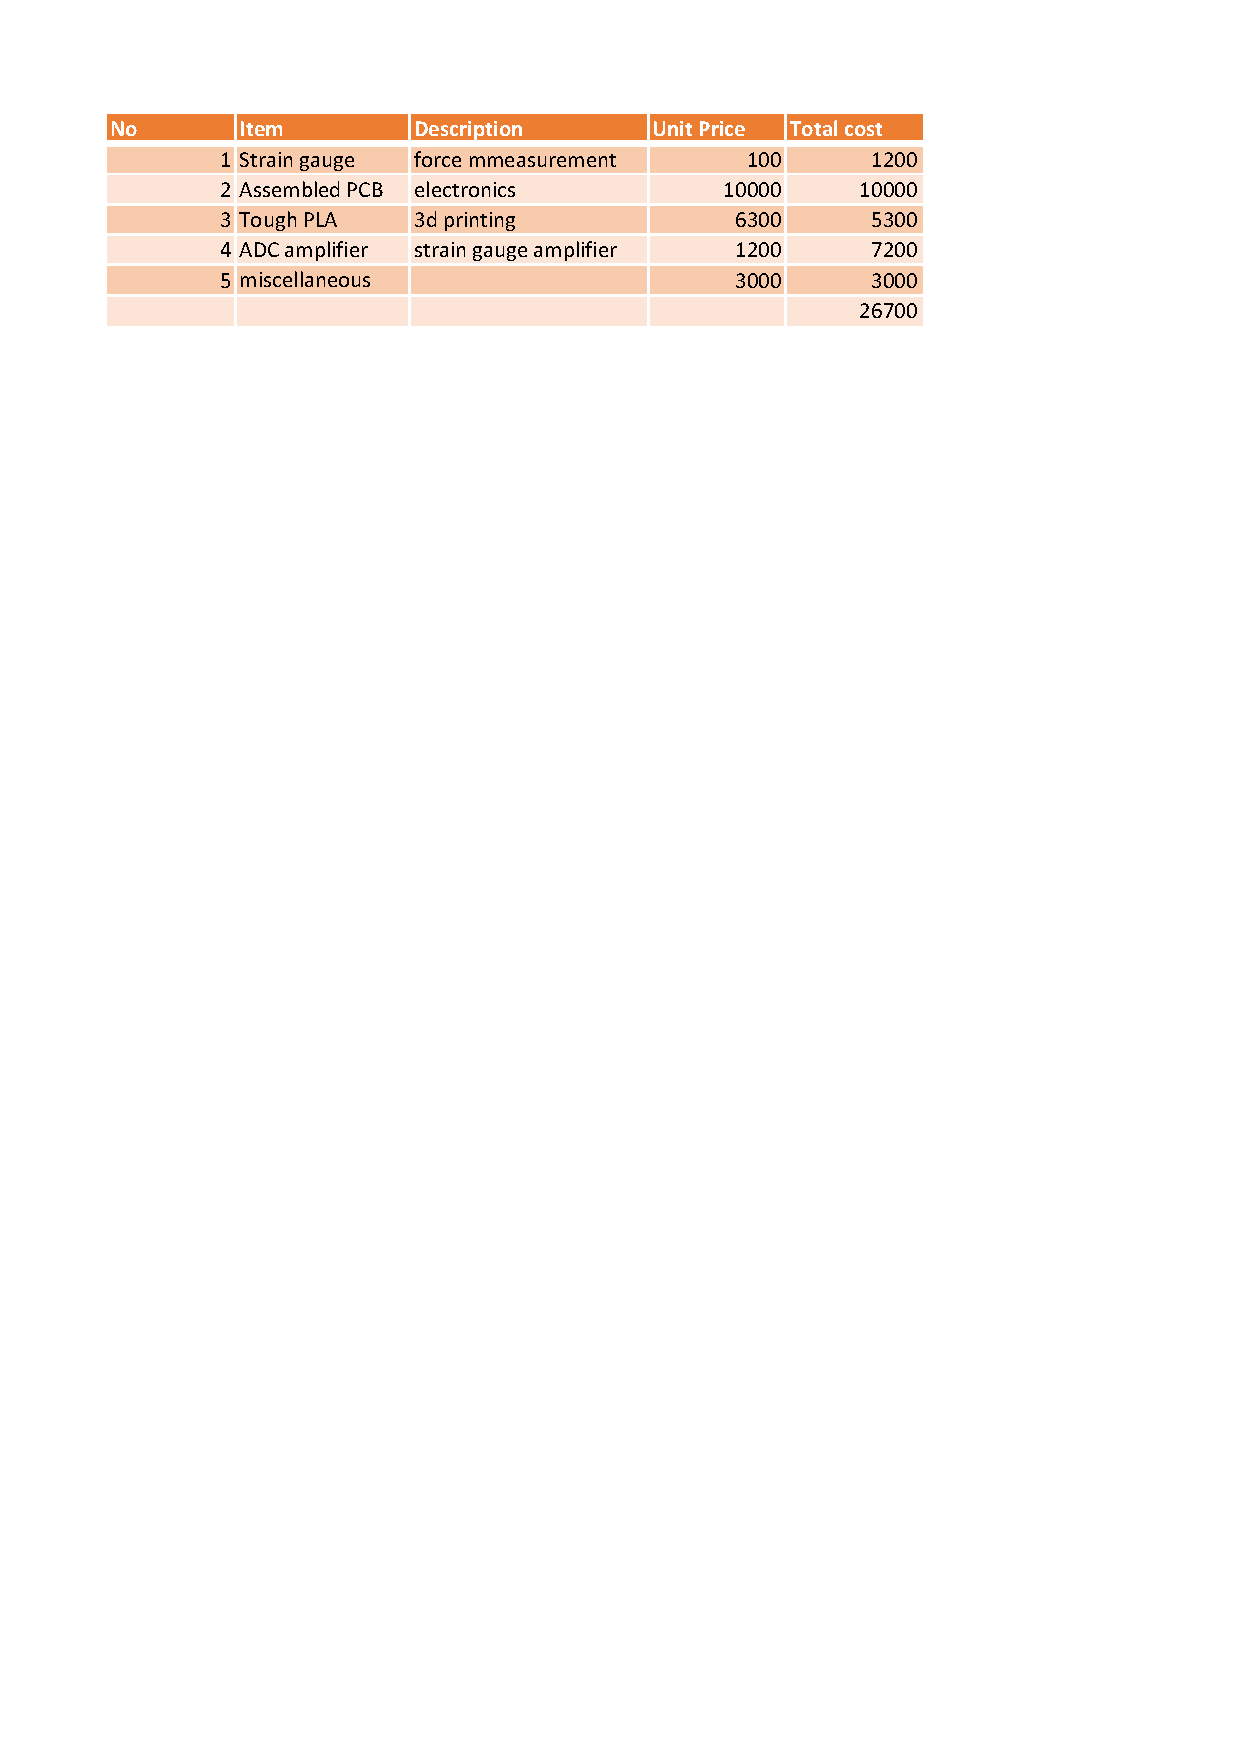
\includegraphics{Figures/budget}
 \end{table}
 \end{center}
 \subsubsection{Work Plan}
 \begin{center}
 \begin{table}[!h]
 \centering
 \caption[Time plan]{Time plan for first and second semester}
 \paragraph{ }
 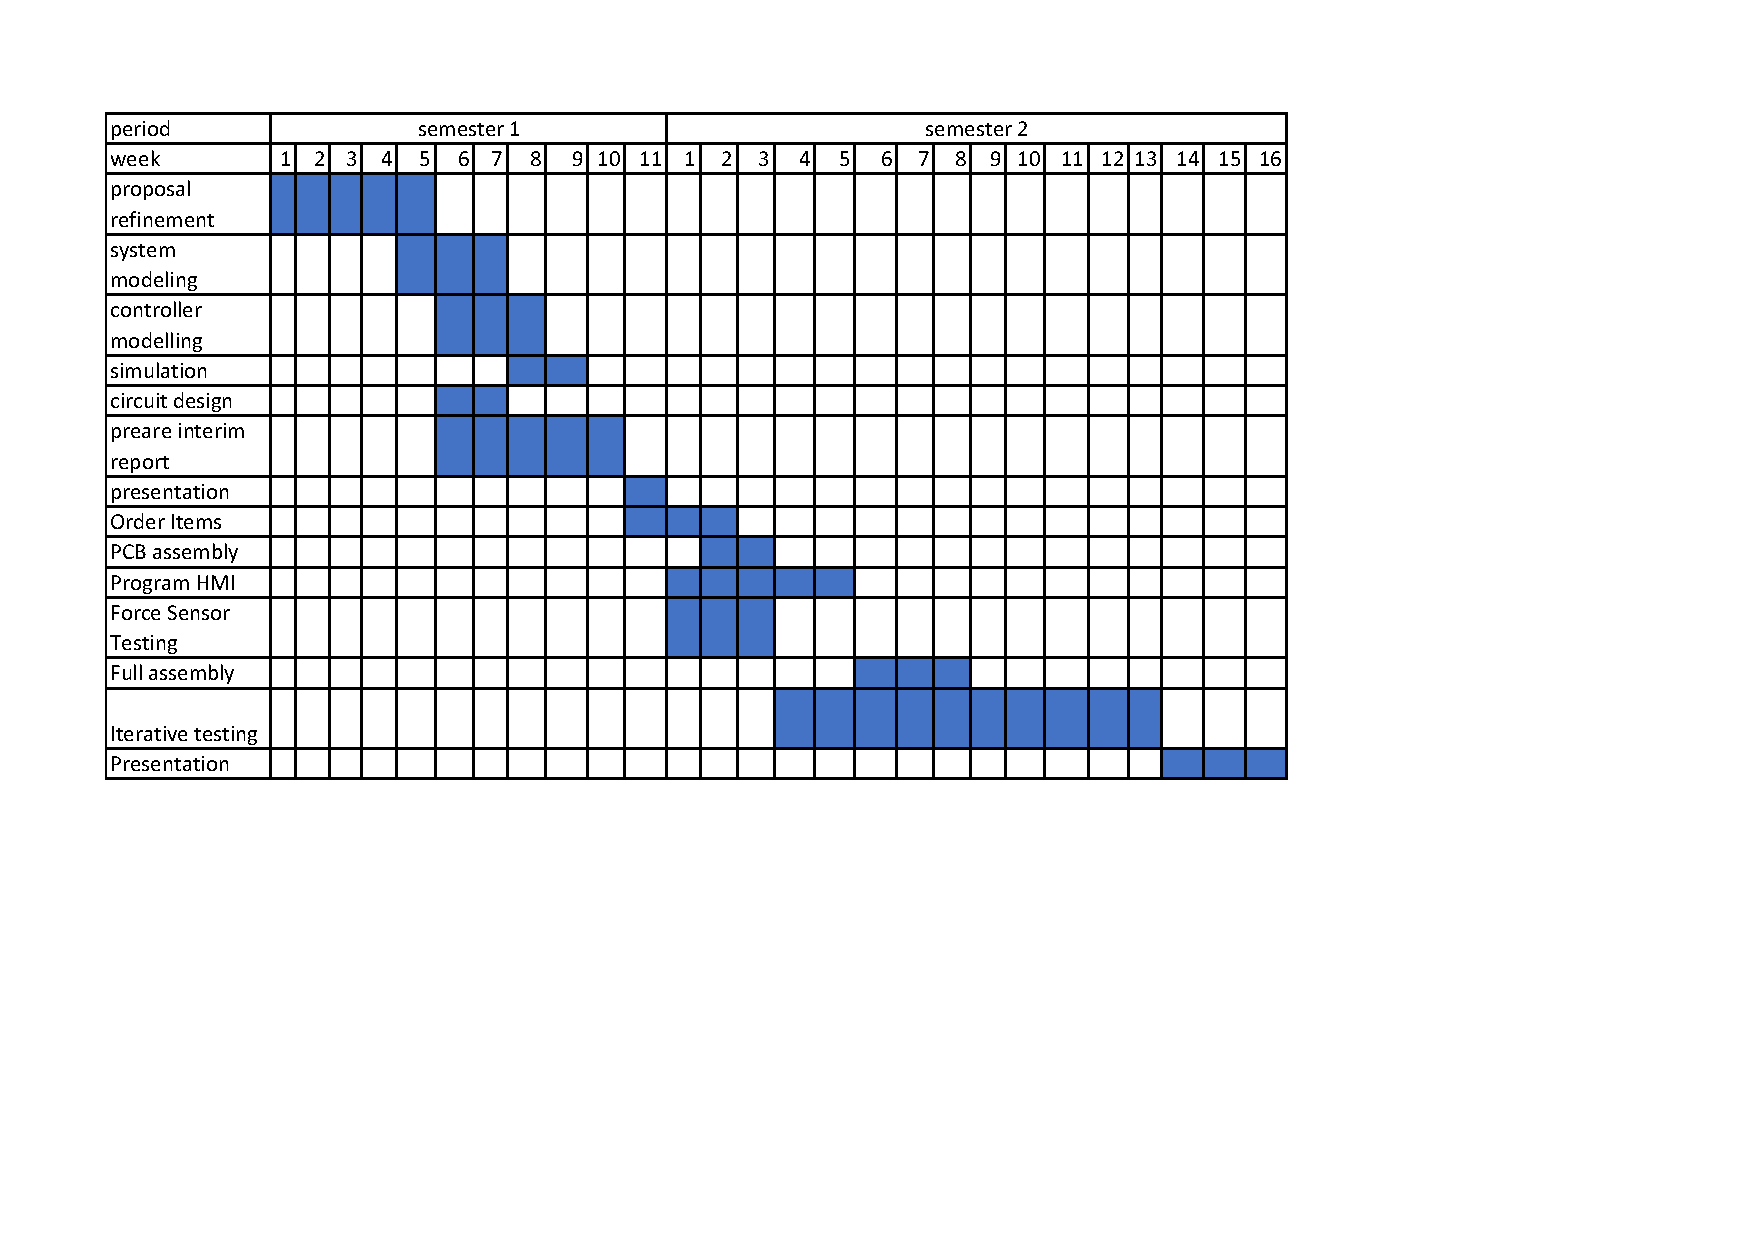
\includegraphics[width=0.95\linewidth]{Figures/workplan}
 \end{table}
 \end{center}
\subsection{HMI code}
 \subsubsection{Program}
 \begin{verbatim}
 package main
 
 import (
 	"fmt"
 	"math"
 
 	g "github.com/AllenDang/giu"
 )
 
 var (
 	yaw         int32
 	pitch       int32
 	roll        int32
 	transx      int32
 	transy      int32
 	transz      int32
 	tabwidth    float32 = 350
 	tabheight   float32 = 150
 	leg1        []float64
 	leg2        []float64
 	leg3        []float64
 	leg4        []float64
 	leg5        []float64
 	leg6        []float64
 	lineTicks   []g.PlotTicker
 	airVelocity []float64
 )
 
 func loop() {
 	g.SingleWindowWithMenuBar().Layout(
 		g.SplitLayout(g.DirectionVertical, tabheight,
 			g.SplitLayout(g.DirectionHorizontal, tabwidth,
 				g.Layout{
 					g.Label("Rotation Angles"),
 					g.Row(
 						g.VSliderInt(&yaw, -5, 5).Label("Yaw").Size(40, 110).OnChange(func() { fmt.Println(yaw) }),
 						g.VSliderInt(&pitch, -5, 5).Label("Pitch").Size(40, 110),
 						g.VSliderInt(&roll, -5, 5).Label("Roll").Size(40, 110),
 					),
 				},
 				g.SplitLayout(g.DirectionHorizontal, tabwidth,
 					g.Layout{
 						g.Label("Translations (mm)"),
 						g.Row(
 							g.VSliderInt(&transx, -5, 5).Label("X").Size(40, 110).OnChange(func() { fmt.Println(yaw) }),
 							g.VSliderInt(&transy, -5, 5).Label("Y").Size(40, 110),
 							g.VSliderInt(&transz, -5, 5).Label("Z").Size(40, 110),
 						),
 					},
 					g.Layout{
 						g.Row(
 							g.Button("Home Platform").Size(120, 100),
 							g.Button("Write Position").Size(120, 100),
 							g.Button("Record Data").Size(120, 100),
 						),
 					},
 				),
 			),
 			g.Layout{
 				g.Plot("Strain Data").AxisLimits(0, 100, -1.2, 1.2, g.ConditionOnce).XTicks(lineTicks, false).Plots(
 					g.PlotLine("Leg 1", leg1),
 					g.PlotLine("Leg 2", leg2),
 					g.PlotLine("Leg 3", leg3),
 					g.PlotLine("Leg 4", leg4),
 					g.PlotLine("Leg 5", leg5),
 					g.PlotLine("Leg 6", leg6),
 				),
 				g.Plot("Air velocity").AxisLimits(0, 100, -2, 2, g.ConditionOnce).XTicks(lineTicks, false).Plots(
 					g.PlotScatter("velocity(m/s)", airVelocity),
 				),
 			},
 		),
 	)
 }
 
 func main() {
 	for x := 0.0; x < 10; x += 0.1 {
 		leg1 = append(leg1, math.Sin(x))
 		leg2 = append(leg2, math.Cos(x))
 		leg3 = append(leg3, math.Sin(x)+0.1)
 		leg4 = append(leg4, math.Cos(x)+0.1)
 		leg5 = append(leg5, math.Sin(x)+0.3)
 		leg6 = append(leg6, math.Cos(x)+0.3)
 	}
 	for x := 0.0; x < 10; x += 0.1 {
 		airVelocity = append(airVelocity, 1.5)
 	}
 	w := g.NewMasterWindow("Overview", 1300, 700, 0)
 	w.Run(loop)
 }
 
 \end{verbatim}
 
 \subsection{PCB schematics}
 \subsubsection{schematics}
 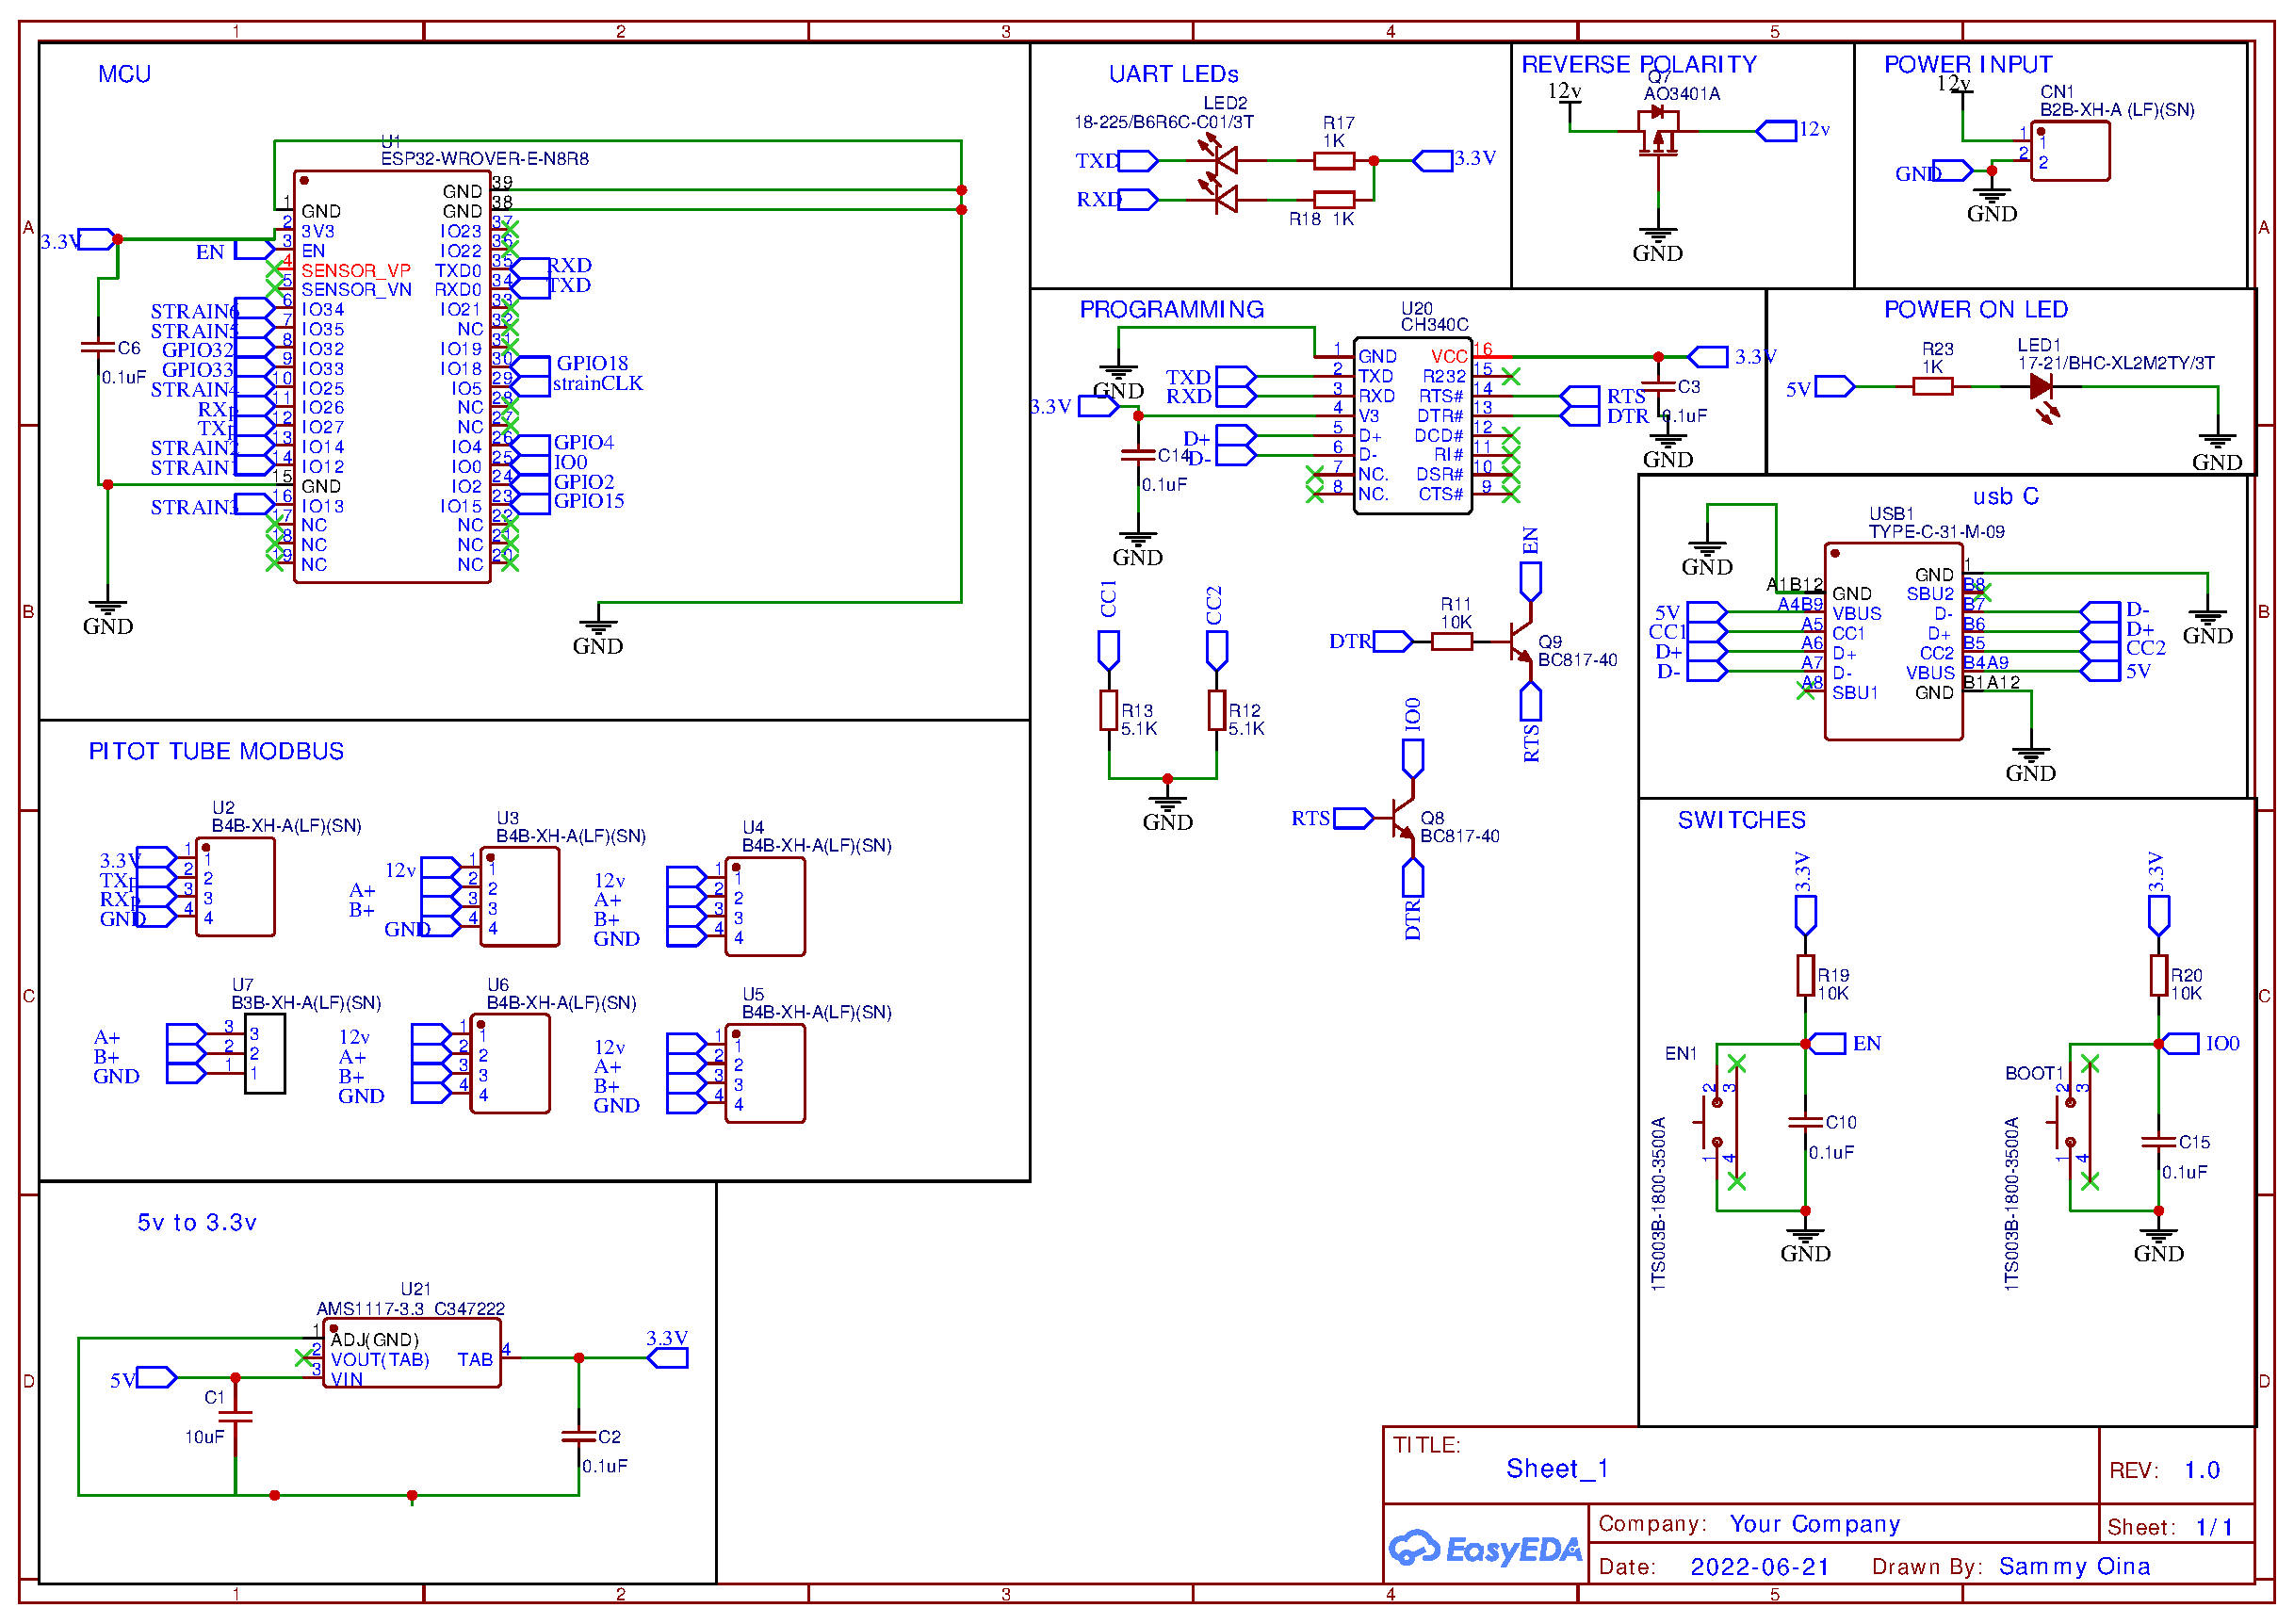
\includepdf[pages=-]{Figures/schm}